\chapter{Compacidad}

\section{Definición y equivalencias}

\begin{definition}
	Sea $X$ un espacio métrico. Decimos que $X$ es \emph{compacto} si todo cubrimiento abierto admite un subcubrimiento finito.
\end{definition}

De cierta forma, los espacios métricos compactos son análogos a los conjuntos finitos. Es decir, muchas de las propiedades de los conjuntos finitos ---tomar mínimo, por ejemplo--- valen también para los compactos.

\begin{definition}
	Decimos que $X$ es \emph{totalmente acotado} si para todo $\varepsilon > 0$, existe un cubrimiento finito con bolas de radio menor o igual a $\varepsilon$.
\end{definition}

\begin{remark}
	Notar la sutileza de la definición. Si bien ser totalmente acotado implica ser acotado, la vuelta no es verdad.
\end{remark}

Damos equivalencias de compacidad.
\begin{theorem}
	Sea $X$ un espacio métrico. Son equivalentes:
	\begin{enumerate}
		\item $X$ es compacto.
		\item Toda sucesión de $X$ admite una subsucesión convergente.
		\item $X$ es totalmente acotado y completo.
	\end{enumerate}
\end{theorem}

\begin{proof}
	(1 $\Rightarrow$ 2) Sea $X$ compacto. Supongamos que existe una sucesión $(x_n)_{n \in \mathbb{N}}$ que no tiene ninguna subsucesión convergente. Por lo tanto, no tiene ningún punto de acumulación. Entonces, para cada $x \in X$, existe un $\varepsilon_x > 0$ tal que $B(x, \varepsilon_x)$ contiene únicamente finitos términos de $(x_n)_{n \in \mathbb{N}}$. Con esto, armamos el cubrimiento abierto $\mathcal{U} = \left\{ B(x, \varepsilon_x) \right\}_{x \in X}$. Por compacidad, existe un subcubrimiento finito. Esto es una contradicción, ya que el subcubrimiento finito cubriría a todos los términos de la sucesión, forzando a alguna de las bolas a contener infinitos términos, contradiciendo la elección de los $\varepsilon_x$.

	(2 $\Rightarrow$ 3) Sea $X$ tal que toda sucesión admite una subsucesión convergente. Para ver la completitud, basta con tomar una sucesión de Cauchy y tomar una subsucesión convergente.
	Veamos la total acotación. Supongamos que $X$ no es totalmente acotado. Entonces, existe $\varepsilon_0 > 0$ tal que no hay un cubrimiento por finitas bolas de radio $\varepsilon$. Construimos una sucesión que no admite una subsucesión convergente. Sea $x_1 \in X$. Sea $x_2 \in X \setminus B(x_1, \varepsilon_0)$. Seguimos inductivamente y obtenemos que $x_n \in X \setminus \left( \bigcup_{i < n} B(x_i, \varepsilon_0)\right)$. Nuestra sucesión cumple que para $i \neq j$, $d(x_i, x_j) \geq \varepsilon_0$. Por hipótesis, $(x_n)_{n \in \mathbb{N}}$ tiene una subsucesión convergente $(x_{n_k})_{k \in \mathbb{N}}$. Sin embargo, $(x_{n_k})$ no es de Cauchy ya que $d(x_{n_{i}}, x_{n_j}) \geq \varepsilon_0$, por ende no es convergente.

	(3 $\Rightarrow$ 1) Sea $X$ totalmente acotado y completo. Sea $\mathcal{U} = \left\{ U_i \right\}_{i \in I}$ un cubrimiento abierto de $X$ tal que no admite un subcubrimiento finito.

	Consideramos al cubrimiento finito por bolas abiertas $\left\{ B(x_n, 1) \right\}_{1 \leq n \leq N}$. Por lo menos una de estas bolas no puede ser cubierta por ningún subcubrimiento finito de $\mathcal{U}$. Llamemos a esta bola $B_1 = B(x_1, 1)$.

	Podemos cubrir a $B_1$ con finitas bolas de radio $\frac{1}{2}$ tales que sus centros distan como mucho a $1 + \frac{1}{2}$ de $x_1$. Por el mismo argumento de antes, una de estas bolas no puede ser cubierta por ningún subcubrimiento finito de $\mathcal{U}$. Llamemos a esta bola $B_2 = B(x_2, \frac{1}{2})$.

	Repetimos el mismo proceso de $B_1$ con $B_2$ y conseguimos la bola $B_3 = B(x_3, \frac{1}{2^2})$. Procediendo inductivamente, obtenemos la sucesión $(B_n)_{n \in \mathbb{N}}$ tal que $d(x_{n-1}, x_{n}) \leq \frac{1}{2^{n-1}} + \frac{1}{2^n}$ para todo $n \in \mathbb{N}$.

	\begin{center}
		
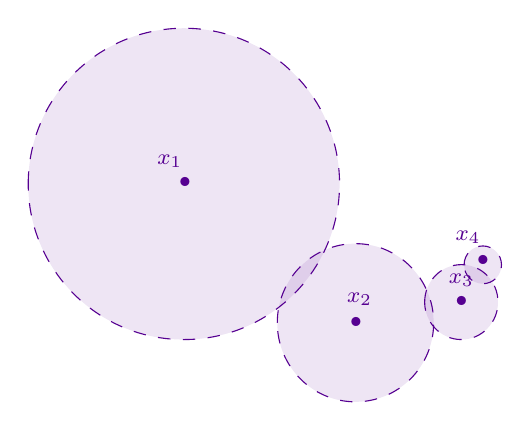
\begin{tikzpicture}[x=0.75pt,y=0.75pt,yscale=-1,xscale=1]
	%uncomment if require: \path (0,300); %set diagram left start at 0, and has height of 300

	%Shape: Ellipse [id:dp7658406221599783] 
	\draw  [color={rgb, 255:red, 86; green, 0; blue, 145 }  ,draw opacity=1 ][fill={rgb, 255:red, 86; green, 0; blue, 145 }  ,fill opacity=0.1 ][dash pattern={on 4.5pt off 4.5pt}] (0,75) .. controls (0,33.58) and (33.58,0) .. (75,0) .. controls (116.42,0) and (150,33.58) .. (150,75) .. controls (150,116.42) and (116.42,150) .. (75,150) .. controls (33.58,150) and (0,116.42) .. (0,75) -- cycle ;

	%Shape: Ellipse [id:dp6629907428161504] 
	\draw  [color={rgb, 255:red, 86; green, 0; blue, 145 }  ,draw opacity=1 ][fill={rgb, 255:red, 86; green, 0; blue, 145 }  ,fill opacity=0.1 ][dash pattern={on 4.5pt off 4.5pt}] (120,141.9) .. controls (120,120.85) and (136.86,103.79) .. (157.67,103.79) .. controls (178.47,103.79) and (195.33,120.85) .. (195.33,141.9) .. controls (195.33,162.94) and (178.47,180) .. (157.67,180) .. controls (136.86,180) and (120,162.94) .. (120,141.9) -- cycle ;
	%Shape: Ellipse [id:dp09734770391428005] 
	\draw  [color={rgb, 255:red, 86; green, 0; blue, 145 }  ,draw opacity=1 ][fill={rgb, 255:red, 86; green, 0; blue, 145 }  ,fill opacity=0.1 ][dash pattern={on 4.5pt off 4.5pt}] (191,131.95) .. controls (191,121.98) and (198.91,113.9) .. (208.67,113.9) .. controls (218.42,113.9) and (226.33,121.98) .. (226.33,131.95) .. controls (226.33,141.92) and (218.42,150) .. (208.67,150) .. controls (198.91,150) and (191,141.92) .. (191,131.95) -- cycle ;
	%Shape: Ellipse [id:dp1342431229797264] 
	\draw  [color={rgb, 255:red, 86; green, 0; blue, 145 }  ,draw opacity=1 ][fill={rgb, 255:red, 86; green, 0; blue, 145 }  ,fill opacity=0.1 ][dash pattern={on 4.5pt off 4.5pt}] (210,114) .. controls (210,108.97) and (214.03,104.9) .. (219.01,104.9) .. controls (223.99,104.9) and (228.02,108.97) .. (228.02,114) .. controls (228.02,119.03) and (223.99,123.1) .. (219.01,123.1) .. controls (214.03,123.1) and (210,119.03) .. (210,114) -- cycle ;

	% Text Node
	\draw (61,60) node [anchor=north west][inner sep=0.75pt]  [font=\footnotesize,color={rgb, 255:red, 86; green, 0; blue, 145 }  ,opacity=1 ]  {$x_{1}$};
	% Text Node
	\draw (75.5,74.5) node  [font=\footnotesize,color={rgb, 255:red, 86; green, 0; blue, 145 }  ,opacity=1 ]  {$\bullet $};
	% Text Node
	\draw (201.4,117) node [anchor=north west][inner sep=0.75pt]  [font=\footnotesize,color={rgb, 255:red, 86; green, 0; blue, 145 }  ,opacity=1 ]  {$x_{3}$};
	% Text Node
	\draw (208.78,131.83) node  [font=\footnotesize,color={rgb, 255:red, 86; green, 0; blue, 145 }  ,opacity=1 ]  {$\bullet $};
	% Text Node
	\draw (152.4,126.08) node [anchor=north west][inner sep=0.75pt]  [font=\footnotesize,color={rgb, 255:red, 86; green, 0; blue, 145 }  ,opacity=1 ]  {$x_{2}$};
	% Text Node
	\draw (157.92,141.64) node  [font=\footnotesize,color={rgb, 255:red, 86; green, 0; blue, 145 }  ,opacity=1 ]  {$\bullet $};
	% Text Node
	\draw (204.61,96.47) node [anchor=north west][inner sep=0.75pt]  [font=\footnotesize,color={rgb, 255:red, 86; green, 0; blue, 145 }  ,opacity=1 ]  {$x_{4}$};
	% Text Node
	\draw (219.07,111.94) node  [font=\footnotesize,color={rgb, 255:red, 86; green, 0; blue, 145 }  ,opacity=1 ]  {$\bullet $};
	% Text Node
	\draw (219,95.5) node  [font=\footnotesize,color={rgb, 255:red, 86; green, 0; blue, 145 }  ,opacity=1 ,rotate=-283.93]  {$\dotsc $};


\end{tikzpicture}

	\end{center}

	Consideramos la sucesión de centros $(x_n)_{n \in \mathbb{N}}$. Sean $m, n, N \in \mathbb{N}$ tales que $N \leq m \leq n$. Entonces,
	\begin{equation*}
		d(x_m, x_n) \leq d(x_m, x_{m+1}) + d(x_{m+1}, x_{m+2}) + \dots + d(x_{n-1}, x_n) \leq \frac{1}{2^{N-2}}.
	\end{equation*}
	Por lo tanto, $(x_n)$ es de Cauchy y como $X$ es completo, tiene límite $x$.

	Sea $U_i$ tal que $x \in U_i$. Dado que $U_i$ es abierto, existe un $r > 0$ tal que $B(x, r) \subseteq U_i$. Por lo tanto, existe un $N \in \mathbb{N}$ tal que $B_{N} \subseteq B(x, r) \subseteq U_i$, lo cual es absurdo por construcción de $(B_n)$.
\end{proof}

Si estamos tratando en $\mathbb{R}^n$, podemos dar una caracterización de compacidad.

\begin{theorem}[Heine–-Borel]
	Sea $A \subseteq \mathbb{R}^n$. Entonces, $A$ es compacto si y sólo si es cerrado y acotado.
\end{theorem}

\begin{proof}
	($\Rightarrow$) Supongamos que $A$ es compacto, es decir completo y totalmente acotado. Veamos que $A$ es cerrado y acotado. Como $A$ es completo, entonces es cerrado y como es totalmente acotado, en particular es acotado.

	($\Leftarrow$) Supongamos que $A$ es cerrado y acotado. Veamos que $A$ es compacto. Basta con ver que toda sucesión de puntos de $A$ admite una subsucesión convergente.

	Sea $(x_k)_{k \in \mathbb{N}}$ una sucesión de puntos de $A$. Como $A$ es acotado, existe un $R > 0$ tal que $B(0, R)$ contiene a todos los puntos de la sucesión. Entonces, por el Teorema de Bolzano–-Weierstrass, existe una subsucesión convergente $(x_{n_k})_{k \in \mathbb{N}}$ que converge a un punto $x \in B(0, R)$. Como $A$ es cerrado, entonces $x \in A$. Por lo tanto, $A$ es compacto.
\end{proof}

\begin{remark}
	Este teorema no es válido en espacios métricos generales. Por ejemplo, el conjunto $\mathbb{Q} \cap [0,1]$ es cerrado y acotado en $\mathbb{Q}$, pero no es compacto, ya que $\mathbb{Q}$ no es completo.
\end{remark}

\section{Propiedades de compactos}

Veamos algunas propiedades de los compactos.

\begin{proposition}
	Sea $X$ compacto e $Y$ un espacio métrico y sea $f : X \to Y$ continua. Entonces, $f(X)$ es compacto.
\end{proposition}

\begin{proof}
	Sea $\left\{ V_i \right\}_{i \in I}$ un cubrimiento abierto de $f(X)$. Consideramos el cubrimiento $\left\{ f^{-1}(V_i) \right\}_{i \in I}$. Dado que $X$ es compacto, consideramos un subconjunto finito $J \subseteq I $ tal que forma un subcubrimiento finito. Ahora consideramos $\left\{ V_j \right\}_{j \in J}$ y vemos que es un cubrimiento de $f(X)$. Sea $y \in f(X)$, entonces existe un $x \in X$ tal que $f(x) = y$. Sabemos que $x \in f^{-1}(V_j)$ para algún $j \in J$. Por lo tanto, $y \in V_j$.
\end{proof}

\begin{proposition}
	Sea $X$ compacto e $Y$ un espacio métrico y sea $f : X \to Y$ continua. Entonces, $f$ es uniformemente continua.
\end{proposition}

\begin{proof}
	Supongamos que $f$ no es uniformemente continua. Es decir
	\begin{equation*}
		\exists \varepsilon > 0 \mid \forall \delta > 0, \exists x, y \mid d(x, y) < \delta \text{ pero } d(f(x), f(y)) \geq \varepsilon.
	\end{equation*}
	Tomamos sucesiones $(x_n)_{n \in \mathbb{N}}$ e $(y_n)_{n \in \mathbb{\mathbb{N}}}$ tales que existe $\varepsilon > 0$ tal que
	\begin{equation*}
		d(x_n, y_n) \to 0 \text{ pero } d(f(x_n), f(y_n)) \geq \varepsilon.
	\end{equation*}

	Por compacidad de $X$, puedo tomar dos subsucesiones convergentes de $(x_n)_{n \in \mathbb{N}}$ e $(y_n)\mathbb{n \in \mathbb{N}}$ que tienden a $x_0$ e $y_0$, respectivamente. Entonces, $d(x_0, y_0) = \lim_{k \to \infty} d(x_{n_k}, y_{n_k}) = 0$, entonces $x_0 = y_0$. Sin embargo, esto implica que $d(f(x_0), f(y_0)) = 0$, lo cual es absurdo ya que $d(f(x_{n_k}), f(y_{n_k})) \to d(f(x_0), f(y_0))$ pero $d(f(x_{n_k}), f(y_{n_k})) \geq \varepsilon$.
\end{proof}

Enunciamos el Teorema de Dini, que de cierta manera nos da una forma de probar convergencia de funciones continuas en espacios compactos dada convergencia puntual más algunas hipótesis adicionales.

\begin{theorem}[Dini]
	Sea $X$ compacto y sea $(f_n)_{n \in \mathbb{N}}$ una sucesión de funciones continuas $f_n : X \to \mathbb{R}$ tal que $f_n \to f$ puntualmente y $(f_n)_{n \in \mathbb{N}}$ es monótona. Entonces $(f_n)_{n \in \mathbb{N}}$ converge uniformemente a $f$.
\end{theorem}

\begin{proof}
	Sin pérdida de generalidad, supongamos que $(f_n)_{n \in \mathbb{N}}$ es monótona creciente. Sea $\varepsilon > 0$. Definimos $g_n = f - f_n$ y consideramos $A_n = g_n^{-1}((-\infty, \varepsilon))$. Como $f_n \to f$ puntualmente, entonces para todo $x \in X$, existe un $n \in \mathbb{N}$ tal que $g_n(x) < \varepsilon$. Por lo tanto, $X = \bigcup_{n \in \mathbb{N}} A_n$.
	
	Notemos también que $A_n$ es abierto, ya que $g_n$ es continua. Por lo tanto, $\left\{ A_n \right\}_{n \in \mathbb{N}}$ es un cubrimiento abierto de $X$. Como $X$ es compacto, existe un subcubrimiento finito $\left\{ A_{n_1}, A_{n_2}, \ldots, A_{n_k} \right\}$ tal que $X = A_{n_1} \cup A_{n_2} \cup \ldots \cup A_{n_k}$.

	Como $(f_n)_{n \in \mathbb{N}}$ es monótona creciente, entonces $(g_n)_{n \in \mathbb{N}}$ es monótona decreciente. Por lo tanto, $A_n \subseteq A_{n+1}$ para todo $n \in \mathbb{N}$. Entonces, $X = A_{n_k}$. Se sigue que, para todo $x \in X$, existe un $n \in \mathbb{N}$ tal que $g_n(x) < \varepsilon$. Es decir, $|f(x) - f_n(x)| < \varepsilon$ para todo $x \in X$ y para todo $n \geq n_k$. Por lo tanto, $(f_n)_{n \in \mathbb{N}}$ converge uniformemente a $f$.
\end{proof}
